\chapter{Conclusion and Interesting Directions}
\label{chap:future}

In this dissertation, we investigated the use of sinusoidal neural networks as digital representations for media objects at multiple resolutions. Neural networks offer a model to approximate continuous functions, bridging the gap between the mathematical universe of modeling and the implementation universe, within the paradigm of the four universes. 

As specialized hardware, such as neural engines and tensor processing units, becomes increasingly integrated into consumer products like laptops, smartphones, smartwatches, virtual reality headsets, and augmented reality glasses, we anticipate that neural assets will play an important role across various industries. Specifically, we foresee a future where neural networks become one of the standard digital representation for assets in domains such as audiovisual content production and gaming.

In this context, this dissertation contributes to the growing body of knowledge by deepening the understanding of frequency behavior in sinusoidal neural networks and its connection to multiresolution analysis theory. We introduced MR-Net, a family of architectures designed to encode signals across multiple resolutions, and showcased its applications to media objects such as images and material textures. Additionally, we demonstrated how to construct periodic sinusoidal neural networks for representing periodic textures, we developed a technique based on the Poisson equation to generate seamless material textures, and we demonstrated how our architectures can be used for rendering textured objects.

Moreover, MR-Net is available as a software library, a flexible Python framework implementing the architectures discussed in Chapter \ref{chap:mr_snn}, along with the multiresolution training process. The framework is publicly accessible at \cite{mrnetGithub}.


Significant progress has been made in this rapidly evolving field, and our work builds upon both contemporary and classical knowledge. However, the contributions presented here mark only the beginning. There remain several key limitations to address and numerous exciting research directions to pursue. These include improving frequency initialization strategies in sinusoidal networks, advancing compression techniques for neural representations, and expanding the scope of applications beyond textures to encompass more complex media objects and materials. We will explore these and other promising avenues in the following sections.

\section{Limitations}

\subsection{Frequencies}

By understanding the relationship between initialization of the first sinusoidal layer of a sinusoidal neural network and the frequencies learned by the model, we have made significant progress into connecting an empirical hyperparameter to the Shannon-Nyquist theory. By introducing integer frequencies, we provided a more structured approach, as these frequencies correspond to a well-defined function space (periodic functions). This allowed us to narrow down the space of possible initialization values to a discrete and finite set, which aids in developing a more principled initialization strategy.

% Moreover, we concluded that using integer frequencies is more appropriate as it has an underlying model that constitutes a representation for a well defined function space (periodic functions) and we can reduce the space of possible values for the initialiation to a discrete a finite set o values, thus helping on the design of a initialization strategy. 
% However, as we discussed in Chapters \ref{ch:imaging} and \ref{chap:seamless-textures}, choosing the best frequencies for initialization or spliting the frequency bands between levels of details remains as empirical task. For the first task, one could say that since the integer frequencies work well, we could choose all the possible choices for a certain bandlimit. However, as a digital represnetation, it is important to keep the network as small as possible. Works like \cite{novello2022understanding} and \cite{tamingFactory} may be a good direction to overcome these challenges.

However, as discussed in Chapters \ref{ch:imaging} and \ref{chap:seamless-textures}, determining the optimal frequencies for initialization or partitioning frequency bands across different levels of detail remains an empirical challenge. While it is tempting to exhaustively select all possible integer frequencies within a given bandlimit, practical constraints, such as the need to maintain a compact network size, demand a more selective approach. Results like those in \cite{novello2022understanding} and \cite{tamingFactory} offer potential solutions to these challenges by exploring more structured approaches to frequency selection.

\subsection{Compression}

% Thinking of a useful digital representation we must make sure it is compact and lightweight to store in the disk or transmiti through the network. Part of this is due to small neural networks architectures, that is, managing to encode signals using networks with less weights. This part was a concern in this dissertation. However, this alone is not sufficient as the size of an image file is not only determided by the amaount of values it has to store, being either the total of pixels in a matrix or the total of weights in a network, but also by the level of compression.

For neural networks to serve as practical digital representations, they must be compact and lightweight for efficient storage and transmission. While this dissertation considered the importance of using networks with minimal weight counts, this alone is insufficient. This task requires not only designing small neural network architectures with fewer weights but also applying effective compression techniques. The file size of a digital representation —whether it be a pixel-based image or a weight-based neural network— is also influenced by the level of compression applied.

For this reason, coupling our results with efficient neural network compression methods, such as those proposed by \cite{dupont2021coin} and \cite{dupont2022coinpp}, or developing novel compression strategies for sinusoidal networks, is crucial for achieving a practical representation that can be efficiently transmitted over networks and stored on disk.


\subsection{Implicit Functions}

Related to the frequencies choice, we would like to discuss the implicit represnetations of media, that is representing an object as a level set of an implicit function. We presented experiemnts for one-dimensional signals, that could be related to audio waves, and image signals. We have also experimented with higher order signals as it will be discussed in \ref{sec:3Dtextures}. However, all these media objects are represented explicitly as scalar or vector fields. In these cases, we can sample the signal uniformly and we have the support of the Shannon-Nyquist theory to guide our choices of initiaization of the networks.

Another possible limitation arises from establishing a relatioship for frequency choices when representing media objects as implicit functions. We presented experiemnts for one-dimensional signals, that could be related to audio waves, and image signals. We have also experimented with higher order signals as it will be discussed in \ref{sec:3Dtextures}. For these cases, we can uniformly sample the signal and leverage the Shannon-Nyquist theory to guide the network's initialization.

However, representing objects implicitly —such as shapes defined by signed or unsigned distance functions— introduces additional complexity. In these cases, the relationship between signal samples and frequencies, as well as techniques for filtering and constructing multiscale representations, is less straightforward. Works like \cite{silva2022mipplicits} show that it is possible and beneficial to decompose implicit signals and represent them using multistage networks, but selecting appropriate hyperparameters remains an uncertain task.

% For objects defined implicitly such as shapes given by a signed distance function or unsigned distance function, the relationship between the samples and the frequencies or even methods for filtering and building a multiscale representation are not straighforward. Works like MIP-PLICITS show that it is possible to and fruitful to decompose these signals and use a multistage network to represent them, but the terrain for choosing hyperparameters may be more unccertain.

Note that NeRF-based methods, that are usually referred as implicit do not fall in this category. Although they are not explicit representations of scenes, they are explicit representation of volume densities. The chalenge in this case comes from learning the volumetric function from 2D data.

It is important to note that NeRF-based methods \citep{2020nerf}, often referred to as implicit representations, do not fall into this category. While they are not explicit scene representations, they represent volumetric densities explicitly. The primary challenge in NeRF-based approaches lies in learning the volumetric function from 2D data, rather than dealing with implicit object representations directly.


\section{Interesting Directions}

\subsection{Volumetric Textures and Hypertextures}
\label{sec:3Dtextures}

Volumetric textures, also known as 3D textures, are defined as vector fields in 3D space. These solid textures offer practical advantages in computer graphics, as they eliminate the need to compute $uv$-coordinates on a surface. Instead, the texture value is directly evaluated at the coordinates $(x, y, z)$.

% Since they are represented explicitly in computer graphics, this looks like a natural extension of the discussion in Chapter \ref{chap:seamless-textures}. We have conducted preliminary experiments in this direction, using the Perlin Noise technique to generate procedural textures of materials like marble (Figure \ref{f:volumetric-texture}). We succcessfully trained a M-Net model to encode a volumetric texture and we managed to integrate it into the omniverse render (Figure \ref{f:volumetric-texture}). However, with this third spatial dimension, the network size increased greatly and we did not think it was worth it, specially in comparison to the procedural representation.

Since volumetric textures are explicitly represented, this extends naturally from the discussions in Chapter \ref{chap:seamless-textures}. We conducted preliminary experiments in this area, using Perlin Noise to generate procedural textures for materials like marble. Our results showed that an M-Net model could successfully encode a volumetric texture, which we integrated into the Omniverse renderer and generated the images in Figure \ref{f:volumetric-texture}. However, incorporating the third spatial dimension resulted in a significant increase in network size, reducing the practicality of this approach compared to procedural methods.

\begin{figure}[h]
   \centering
   \begin{subfigure}[b]{0.32\textwidth}
       \centering
       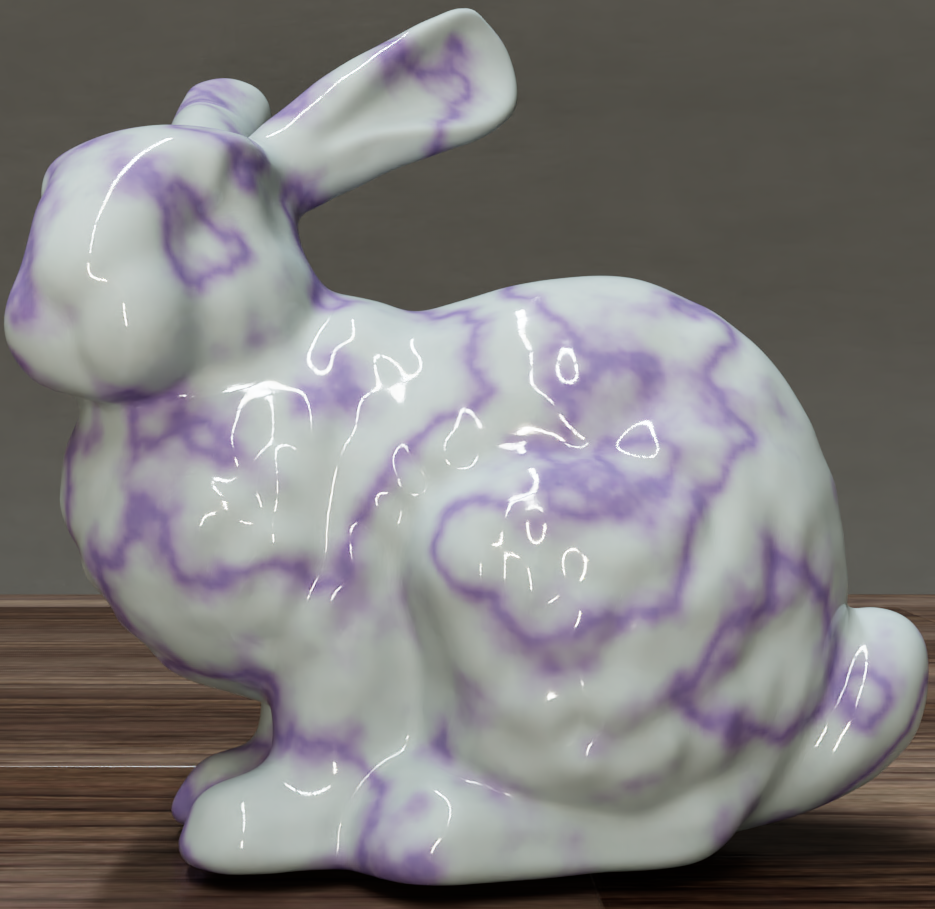
\includegraphics[width=\textwidth]{img/ch7/bunny_mrnet.0000.png}
       \caption{}
   \end{subfigure}
   \begin{subfigure}[b]{0.32\textwidth}
       \centering
       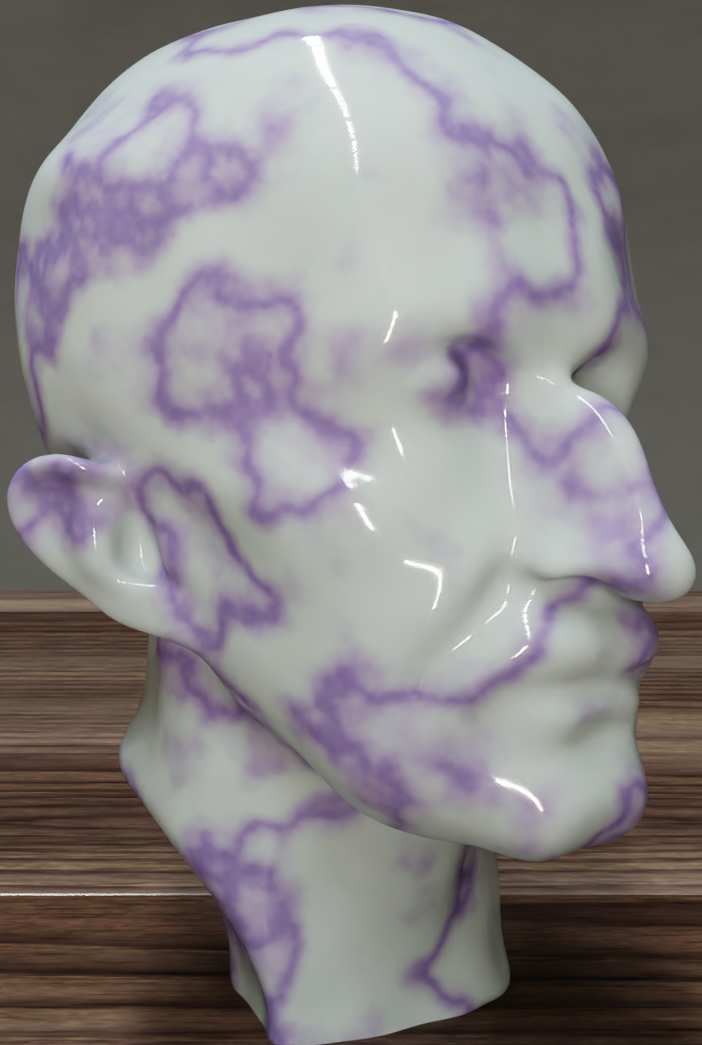
\includegraphics[width=\textwidth]{img/ch7/max_plank_mrnet_512_mc400.0099.png}
       \caption{}
   \end{subfigure}
   \begin{subfigure}[b]{0.32\textwidth}
       \centering
       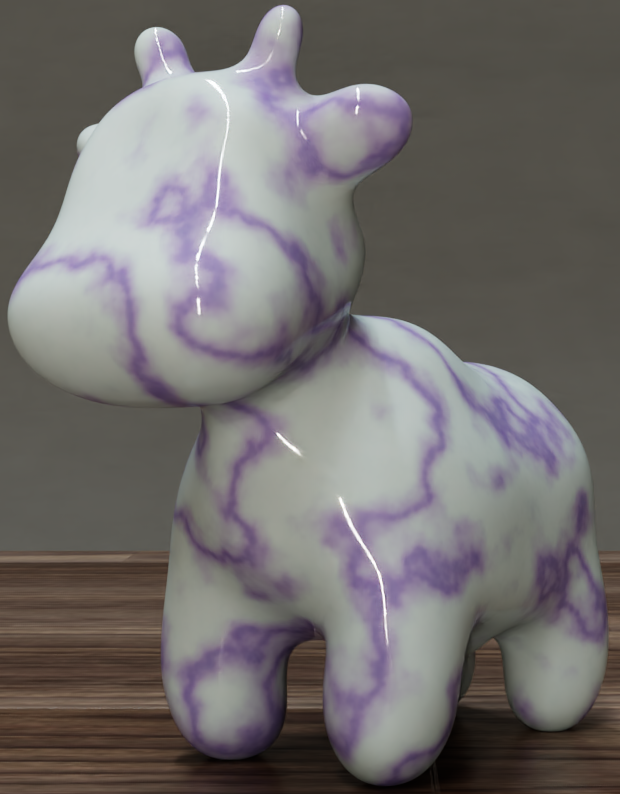
\includegraphics[width=\textwidth]{img/ch7/spot_mrnet.0101.png}
       \caption{}
   \end{subfigure}
   \caption{Volumetric marble texture encoded in a M-Net model and mapped in three different objects. Visualization rendered using the Nvidia Omniverse platform.}
   \label{f:volumetric-texture}
\end{figure}

One future research, thus, would be to investigate further how to optimize the training of MR-Net instaces in this case. Another promising research would be to generate a volumetric texture based on a 2D pattern. The ideia is to design a loss function or add the minimal information necessary to optimize it without requiring a large dataset, pretty much how the seamless texture generation in Chapter \ref{chap:seamless-textures} works.

Future work could focus on optimizing the training of MR-Net instances for volumetric textures. A fractal-based novel architecture could also be devised as a representation for procedural patterns or to optimize a procedural approximation of natural patterns. Another promising direction is to generate volumetric textures from a 2D pattern. A potential research goal would be to design a loss function that allows the network to infer volumetric textures from minimal information, similar to the seamless texture generation process discussed in Chapter \ref{chap:seamless-textures}.

% Another interesting and particular object in computer graphics are the Hypertextures~\citep{hypertexture}. These objects model phenomena intermediate between shape and texture by using space-filling applicative functions to modulate density. The model is essentially an extension of procedural solid texture synthesis, but evaluated throughout a volumetric region instead of only at surfaces. Having a neural representation of this kind of phenonema to address for example fur or hair may be a path to efficient representation of these delicate objects. leveraging the versatility of vector fields in combination with surface representations, holds great potential.

Additionally, hypertextures~\citep{hypertexture}, which model phenomena at the boundary between shape and texture by modulating density with space-filling functions, are another interesting avenue. This technique extends procedural solid texture synthesis to volumetric regions, rather than limiting it to surfaces. Developing neural representations for such phenomena, such as fur or hair, could lead to efficient representations of these complex objects by leveraging vector fields in combination with surface representations.


\subsection{Irregular sampling}

% The input for the neural network is a discrete representation. In this sense, sampling is a way to create a representation of a function based on its values at certain points of the domain. We presented many results based on regular sampling or uniform sampling, for which we have the Shannon-Nyquist theory as support. However, there are many scenarios where irregular sampling may be desirable.

Neural networks rely on discrete input representations, which are created by sampling a continuous function at specific points. In this dissertation, we used regular or uniform sampling, guided by the Shannon-Nyquist theory. However, many scenarios may benefit from irregular sampling techniques.

% First, for objects defined implicitly as level sets of implicit functions, for example shapes given by signed distance functions, we may not have an easy mechanism to define regular sampling and generate samples with these properties. Thus, irregular sampling is the default in this scenario.

For objects implicitly defined as level sets of a function (e.g., shapes given by signed distance functions), regular sampling may not be feasible, making irregular sampling the default. Additionally, even when signals are explicitly represented, as in the one-dimensional cases discussed in Chapter \ref{chap:sinusoidal}, certain points, such as maxima, minima, or inflection points, are more informative than others. We could decide to intentionally look for these points and maybe even use higher order features like the derivatives to train a representational model of this signal. In a multiresolution context, a stratified sampling strategy may be particularly useful. 

% Besides that, even in a scenario where we havean explicit representation of a signal, for example the one-dimensional signals we used in Chapter \ref{chap:sinusoidal}, it is evident that some points are features more important than others. For example, the critical points, those of maxima and minima (or saddle in higher dimensions) or inflection points are very relevant features for signal encoding. For this reason, we could decide to intentionally look for these points and maybe even use higher orther features like the derivatives to train a representational model of this signal. Moreover, thinking in terms of multiresoltion, we could have a stratified staregy of sampling.Furthermore, we believe that the capacity-based level of detail could benefit greatly of an irregular sampling scheme like, for example, the Poisson disk sampling \citep{stochastic_cook}.


In \citet{spectralPoster24} an ideia of using periodic neural networks to encode equirectangular panoramas is presented. In this case, there's a inherent challenge of dealing with the nature of this spherical representation that is periodic in one direction, but not in its orthogonal direction. However, we believe it is possible to derive efficient representations of panoramas like this by leveraging an adaptive sampling grid as in Figure \ref{f:inr-panorama}, taking into account the fact that the equirectangular representation is oversampled in the poles.


\begin{figure}[!ht]
   \centering
   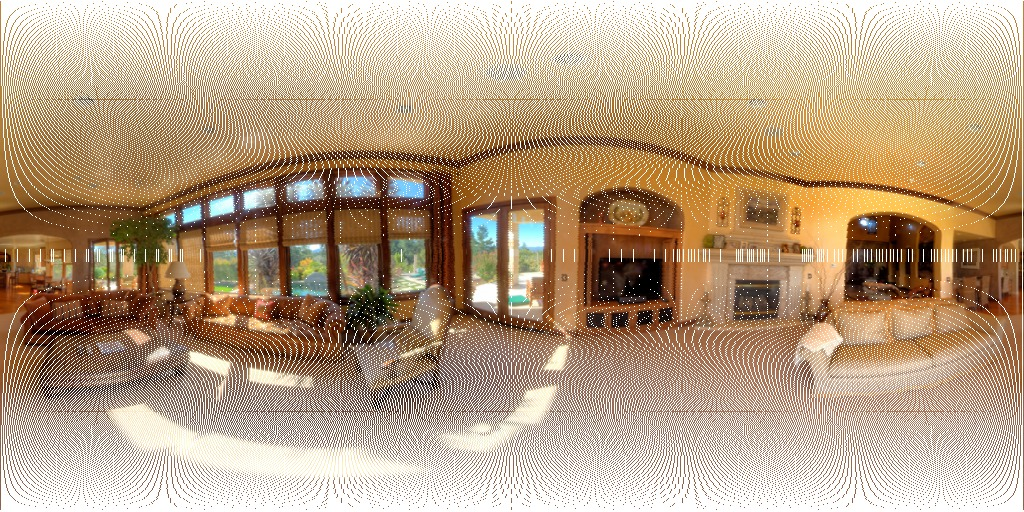
\includegraphics[width=0.80\linewidth]{img/ch7/sampling-pattern.jpeg}
   \caption{Sampling pattern for equirectangular panorama} 
   % \Description[Metric-aware sampling pattern for equirectangular panorama]{Metric-aware sampling pattern for equirectangular panorama}
   \label{f:inr-panorama}
\end{figure}


When dealing with irregular sampling, we do not have aliasing, but we may have noise. Having a mechanism of filtering or not producing this noise when training the representational model is an interesting research direction. In this context, capacity-based level-of-detail schemes could also benefit from irregular sampling patterns, such as Poisson disk sampling \citep{stochastic_cook}.

\subsection{Parameterizing Operations}


Thus far, we have focused on neural representations of media objects as a whole. However, another important direction is the development of methods for manipulating and editing these representations. The functional structure of sinusoidal neural networks provides opportunities to explore algebraic operations for network manipulation.


Neural networks can also be used to represent transformations in a space. For example, \cite{schardong2024neural} used sinusoidal neural networks to model images of human faces and to parameterize morphing transformations between two faces, allowing the generation of a third face that blends features of both individuals in a controlled manner.


% However, neural networks may be used to represent transformations in a space too. For instance, \cite{schardong2024neural} used sinusoidal neural networks to represent images of faces of people and also to parameterize morphing transformations between pairs of people so that it is possible to generate a third face that combines features of both individuals in a controlled manner.


We may go a step further a think that a media content may be interpreted as a single piece or decomposed in multiple subparts. For example we could represent a character moving in a scene as a video or as a sparse set of images and specific transformations between them. This may be lead to a storage efficient way of encoding some videos. Regressing a little bit, this strategy could be used in the sense of optical flow \citep{alfarano-opticalflow} to provide a general neural video format.

This approach could be extended further. Instead of representing a piece of media as a single entity, it could be decomposed into multiple sub-parts. For instance, a character moving in a scene could be represented as a sparse set of keyframes, with specific transformations interpolating between them. This approach could lead to more storage-efficient video representations. In a broader sense, such a strategy could be applied to neural video encoding, possibly leveraging concepts like optical flow \citep{alfarano-opticalflow} to develop a general neural video format.


\section{Final Reflection}

\red{a ser proferida com inspiração}

% We have described a flexible method of working with signals in multiresolution in terms of multiple ways of preparing the input data, defining the MR-Net subclasses, and training multi-stage networks. In the applications presented in Sec. \ref{s:img}, we have explored a subset of this framework, showing cases where it improves upon existing state of the art techniques. Regarding other aspects of this groundwork, we have ongoing research on signal reconstruction from stochastic sampling, and training of L-Net models using the Laplacian pyramid, which may lead to novel imaging applications.  Some of the motivation and experiments with 1D signals in these directions are documented in \citet{supplemental}.


% In terms of future work, we plan to expand this research in two main directions. On one hand, we would like to explore the MR-Net architecture for other image applications including super-resolution, operations in the gradient domain, generation of periodic and quasi-periodic patterns, as well as image compression.
% On the other hand, we would like to extend the MR-Net representation to other media signals in higher dimensions, such as video, volumes, and implicit surfaces.